\subsubsection{Return paths between the MSD and LSD in different rows}

The gadgets of this class hold a increment/copy signal.
The height of these gadgets is dependent on $l$ and the width is dependent of $k$.
These gadgets are used to begin reading the first digit in the following row, once
the MSD has been read in the current row.
\vspace{1cm}

\begin{figure}[H]
    \centering
    \begin{subfigure}[t]{0.3\textwidth}
        \centering
        \includegraphics[width=0.3\textwidth]{return_paths/return_digit1_read_next_row}
        \caption{\label{fig:return_paths/return_digit1_read_next_row} Case -- 1}
    \end{subfigure}%
    ~
    \begin{subfigure}[t]{0.3\textwidth}
        \centering
        \includegraphics[width=0.3\textwidth]{return_paths/return_digit2_read_next_row}
        \caption{\label{fig:return_paths/return_digit2_read_next_row} Case -- 2}
    \end{subfigure}%
    ~
    \begin{subfigure}[t]{0.3\textwidth}
        \centering
        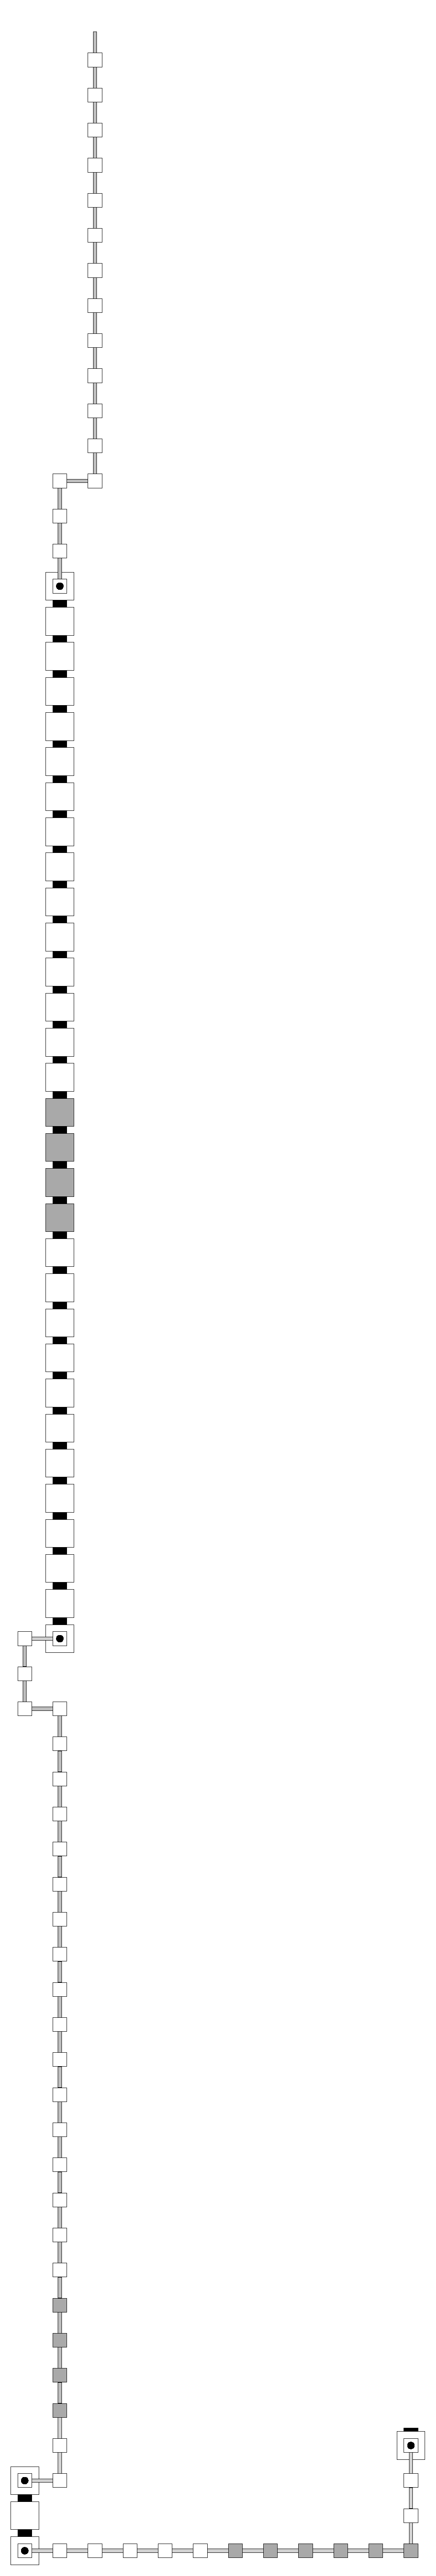
\includegraphics[width=0.3\textwidth]{return_paths/return_digit3_read_next_row}
        \caption{\label{fig:return_paths/return_digit3_read_next_row} Case -- 3}
    \end{subfigure}%
    \caption{\label{fig:return_path_next_row}
    All of these gadgets assemble north to south. The vertical gray lines tiles have a height
    that depends on $l$ and the horizontal gray lines depend on $k$. (cases 1 and 2 are geometrically equivalent)}
\end{figure}


\noindent For each {\inc} $\in \{ {\tt increment, copy } \}$

\begin{itemize}
    \item Create
    $\begin{aligned}[t]
        \returnfromdonereadnextrow(& \left \langle {\tt ReturnD1ReadNextRow},     \inc \right\rangle, & \\
                                    & \left \langle {\tt DigitReader}, 1, \lambda, \inc \right\rangle \;)
    \end{aligned}$

    \item Create
    $\begin{aligned}[t]
        \returnfromdtworeadnextrow(& \left \langle {\tt ReturnD2ReadNextRow},     \inc \right\rangle, & \\
                                    & \left \langle {\tt DigitReader}, 1, \lambda, \inc \right\rangle \;)
    \end{aligned}$

    \item Create
    $\begin{aligned}[t]
        \returnfromdthreereadnextrow(& \left \langle {\tt ReturnD3ReadNextRow},     \inc \right\rangle, & \\
                                        & \left \langle {\tt DigitReader}, 1, \lambda, \inc \right\rangle \;)
    \end{aligned}$
\end{itemize}
\vspace{1cm}